\documentclass{article}
\usepackage[utf8]{inputenc}
\usepackage[spanish]{babel}
\usepackage{listings}
\usepackage{graphicx}
\graphicspath{ {images/} }
\usepackage{cite}

\begin{document}

\begin{titlepage}
    \begin{center}
        \vspace*{1cm}
            
        \Huge
        \textbf{Parcial2}
            
        \vspace{0.5cm}
        \LARGE
        Subtítulo
            
        \vspace{1.5cm}
            
        \textbf{Nombres y Apellidos del autor}
        \newline Julián David Quintero Marín
        \newline
        \newline
        Informática II
        \vfill
            
        \vspace{0.8cm}
            
        \Large
        Despartamento de Ingeniería Electrónica y Telecomunicaciones\\
        Universidad de Antioquia\\
        Medellín\\
        September de 2021
            
    \end{center}
\end{titlepage}

\tableofcontents
\newpage
\section{Análisis del problema y busqueda de soluciones para el programa.}\label{intro}
En este trabajo se busca la forma de mostrar la bandera de cualquier pais del mundo, usando una matriz de led RGB.
Para la solucion del problema, en mi caso reconstruí el código que habían explicado los profesores en clase. En parte si entendí cómo usar los leds y cómo obtener la informacion de cada uno de estos en un punto específico. Ahora el reto es cómo hacer el sobremuestreo y el submuestreo. En este momento no tengo certeza de cómo hacer estas funciones, pero una idea que vi investigando por internet decía que obtener el cociente de la división del ancho de la imagen entre el número de columnas de la matriz de Neopixeles o de LEDs, y de forma similar el alto entre el número de filas, para, posteriormente, usar estos dos valores, para hallar el promedio de un número de valores (Teniendo en cuenta que pueden ser diferentes dependiendo de cúal de los 3 colores RGB esté analizando matricialmente) y así reducir ese número a 1, y unir todas los valores resultantes hasta crear la versión submuestreada de la matriz.
  \begin{figure}[h]
    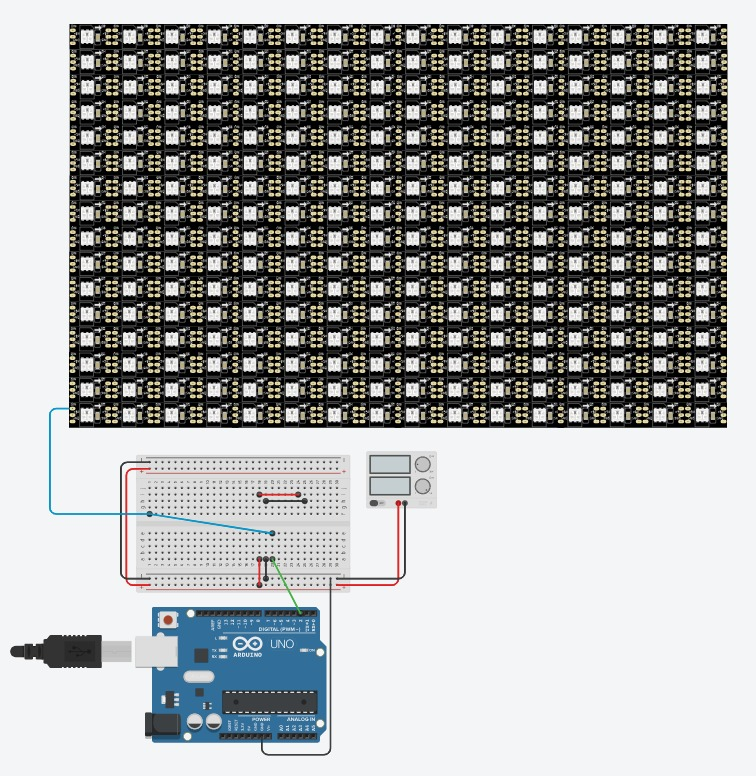
\includegraphics[width=10cm]{matriz_16x16.jpg}
    \centering
    \caption{Construcción de matriz 16x16 de Neopixeles}
    \label{fig:matriz16x16Neopixeles}
 \end{figure}
 \begin{figure}[h]
  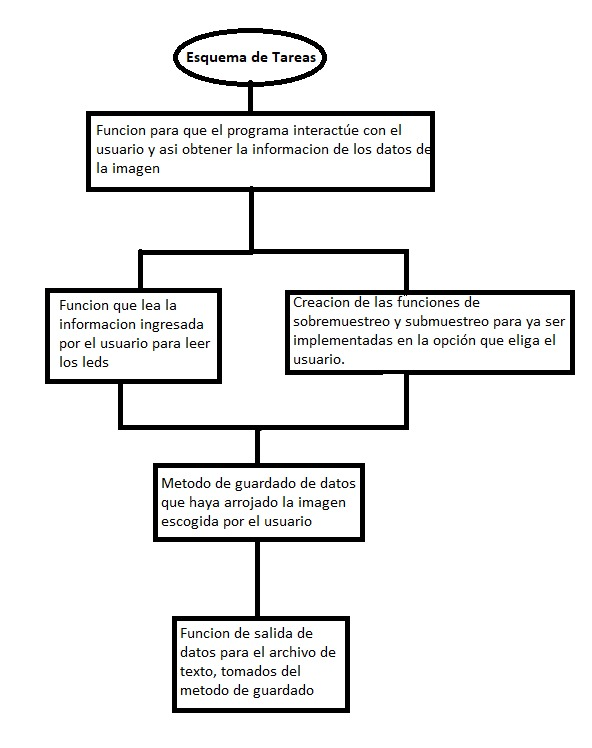
\includegraphics[width=10cm]{Esquema_tareas.jpg}
  \centering
  \caption{Esquema de tareas}
  \label{fig:esquema_tareas}
\end{figure}
\section{Esquema de tareas para el desarrollo del algoritmo} \label{contenido}
1. Para empezar, debemos analizar la lista de tareas que se deben ejecutar para desarrollar el algoritmo de solución del desafío de manera funcional y efectiva. Analizando objetivos de forma secuencial, considero que, primero, es fundamental establecer el método de interacción con el usuario para solicitar la imagen a procesar, por lo cual, una parte de ello, consta de la creación del manual de uso del programa., que debe abordar a su vez, lo que debe hacer el usuario con el archivo de texto resultante del submuestreo o sobremuestreo de la imagen (En caso de que sea alguno de los 2 necesario), incluyendo cómo y dónde debe usarlo, pues dicho archivo contiene la información necesaria para que funcione correctamente la solución implementada en Tinkercad (Primera impresión de cómo debe conectarse Tinkercad y Qt). Una vez hechas las partes de interacción con el usuario, la siguiente tarea corresponde a crear un método de lectura de la información de la imagen y proveer una forma, mediante código, de guardar dicha información de modo que resulte cómoda de usar al procesarla para la cuestión de submuestreo o sobremuestreo de la imagen. Posterior a ello, debo definir métodos que me permitan manipular la información almacenada. Después, es necesario definir métodos, ciclos y ejecuciones necesarias para el caso en que se requiera realizar submuestreo de la imagen, en paralelo con aquellos necesarios para el caso de sobremuestreo de la imagen. Es necesario, después, garantizar métodos así para guardar la nueva información procesada de la imagen en conjunto con la manipulación del archivo de texto. Asimismo, otra tarea fundamental, la cual puede hacerse en paralelo con el proceso anteriormente descrito, radica en la construcción de la matriz de Neopixeles de modo que sea funcional, en primera instancia, y posterior a que ésto se garantice, priorizar la efectividad en la representación matricial de la información procesada de la imagen obtenida por vía del archivo de texto creado y modificado. Esta última tarea, se debe subdividir en la garantización de la representación matricial para cada uno de los colores RGB por separado como primer objetivo y, después, en conjunto.


\section{Diseño del Algoritmo} \label{contenido}
1. 
\newline
\section{Consideraciones a tener en cuenta en la implementación del algoritmo} \label{contenido}
1.  Al analizar la alternativa de solución propuesta y su respectivo algoritmo, considero que uno de los mayores problemas en la implementación, corresponde al uso excesivo de memoria para el guardado de información de los valores enteros por color de cada pixel de la imagen, por lo cual es fundamental buscar métodos en las clases ya integradas en Qt que permitan la modificación de pixeles en la misma imagen de modo que sea innecesario el uso de memoria adicional para realizar el proceso de submuestreo o de sobremuestreo de la imagen. Dado caso de que esto no sea posible en mediana o completamente, hay que proceder al análisis de la utilidad de cada contenedor que provee C++ tanto para la parte del procesamiento de la imagen, cuyo algoritmo está planteado de modo que se fundamenta tanto en la búsqueda como modificación de los elementos de la matriz que abarca los valores enteros de rojo, verde y azul que posee la imagen; así como para las cuestiones de guardado y fácil acceso a los valores enteros finales que van a ser escritos en el archivo de texto y utilizados como referencia para configurar cada uno de los neopixeles de la matriz construida en el proyecto de Tinkercad. Otra de las consideraciones a tener en cuenta, es mantener por separadas las funciones y métodos que sean empleadas para las cuestiones de procesamiento de la imagen aparte de aquellas usadas para la creación del archivo de texto y escritura de los valores enteros dentro de la matriz, con el fin de mantener un mejor orden dentro de las funciones que cumplen los archivos que componen el proyecto en Qt. Del mismo modo, al tratarse de lógicas parecidas pero en últimas distintas, es fundamental que el análisis que conlleva el procesamiento de la imagen, cuando se emplea su sobremuestreo, sea separado por funciones del análisis que se requiera hacer un submuestreo. Por último, lo más fundamental es procurar que los elementos de la segunda clase, la que se encarga del guardado de los valores enteros finales de cada color de cada pixel, posea los elementos privados que sean útiles tanto para cumplir con su principal objetivo como aquellos que sean manejados más como herramientas auxiliares en el procesamiento de los datos de la imagen, que son obtenidos y modificados gracias a la primera clase instaurada.
\newline


\bibliographystyle{IEEEtran}
\bibliography{references}

\end{document}
